\section{Introduzione}
\subsection{Descrizione del dominio}
Il dominio in cui si sta operando è quello dei fagioli, in particolare quello
delle loro varietà: ogni varietà di fagiolo ha, infatti, specifiche
caratteristiche che la contraddistinguono e che possono essere usate per
identificarle.

Lo studio di questo dominio ha importanti applicazioni pratiche, in 
quanto i fagioli secchi sono uno dei legumi più coltivati al mondo e la loro
coltivazione è fortemente legata alle loro varietà. 
Il processo di classificazione è, però, molto spesso svolto a mano 
da personale addetto e richiede quindi un alto costo e molto tempo.
Un modello di Machine Learning permetterebbe
quindi sia di velocizzare la selezione dei fagioli che di ridurre i costi.

\begin{Figure}
    \centering
    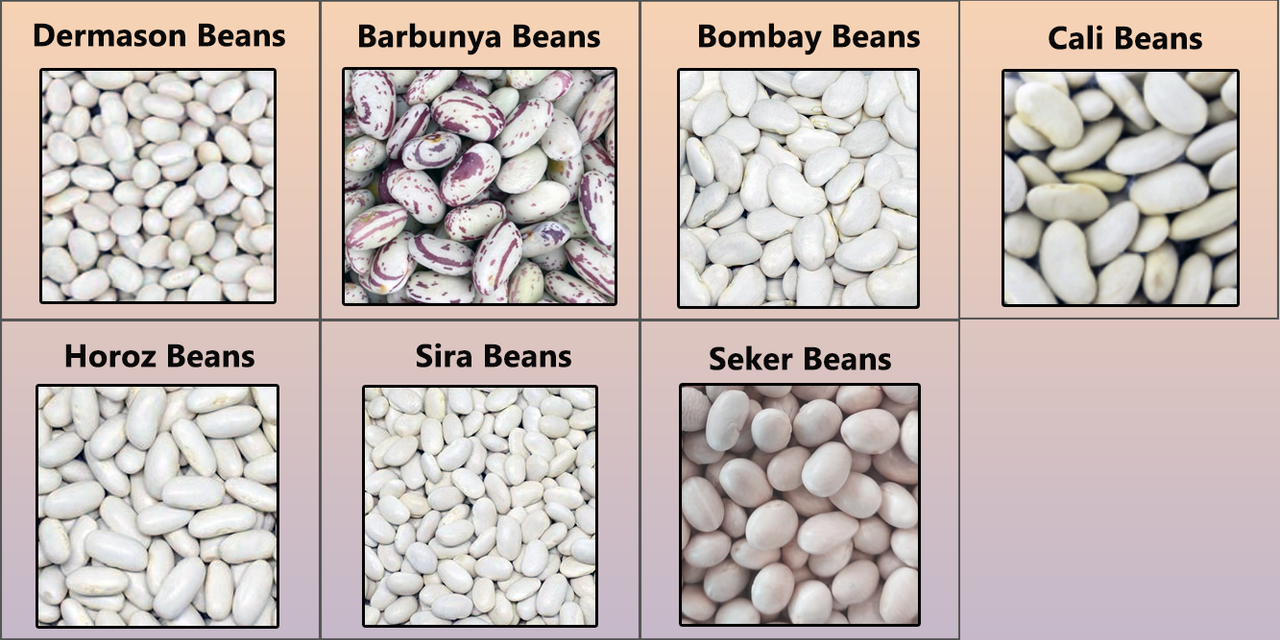
\includegraphics[width=\linewidth]{img/dry_beans.png}
    \captionof{figure}{Varietà di fagioli considerate.}
\end{Figure}

Il dominio analizzato si concentra su sole sette varietà di fagioli, in quanto
quelle più conosciute e interessanti agli autori originali del dataset:
Seker, Barbunya, Bombay, Cali, Dermosan, Horoz e Sira.

\subsection{Creazione del dataset}
Il dataset \cite{dry_bean_dataset} qui considerato è stato creato sfruttando un
sistema di computer vision, appositamente sviluppato per questo dominio
dai suoi autori originali: ogni fagiolo è stato, quindi, inquadrato 
singolarmente e ne è stata così ottenuta un'immagine in alta definizione.
A partire da ogni immagine, poi, il sistema ha effettuato segmentazione
e feature extraction: questo passaggio permette di evitare di trattare
i fagioli tramite i singoli pixel delle immagini che li rappresentano,
rendendoli analizzabili sfruttando molti meno dati ma più significativi,
come forma e dimensioni.